\documentclass[10pt]{article}
\usepackage[margin=0.7in]{geometry}
\usepackage{amsmath,amssymb}
\usepackage{graphicx}
\usepackage{booktabs}
\usepackage[numbers,sort&compress]{natbib}
\usepackage{url}
\usepackage[font=small,labelfont=bf]{caption}
\usepackage{titlesec}
\titlespacing*{\section}{0pt}{6pt}{2pt}
\setlength{\textfloatsep}{8pt plus 2pt minus 2pt}
\setlength{\abovedisplayskip}{4pt}\setlength{\belowdisplayskip}{4pt}
\setlength{\parskip}{2pt}
\graphicspath{{figures/}}

\newcommand{\bv}[1]{\mathbf{#1}}

\title{\vspace{-1.6em}Stabilising a Physics-Informed Neural Network for Pigeon-Flock Interaction Laws\vspace{-0.4em}}
\author{CEE 292 Course Project}
\date{\vspace{-1.2em}}

\begin{document}
\maketitle

\noindent\textbf{Summary.}
This project reproduces the physics-informed neural network (PINN) of Kim et al.~\cite{kim2025}, which infers a pairwise interaction law from the trajectories of a ten-pigeon flock~\cite{nagy2010}, and tests the inferred law as a forward model by simulating the flock for 140\,s.
Three changes were tried: a hard initial condition, self-adaptive loss weights, and constraints on the learned force law (a bounded long-range tail, a minimum pull toward neighbours and each bird's own cruising speed).
The hard initial condition lowered the training loss and doubled the success rate, but 8 of its 10 learned laws blow up in simulation; the adaptive weights traded the trajectory fit for the physics residual and 8 of 10 flocks broke away from their leader.
Only the force-law constraints improved the simulation: no blow-ups (against 2 of 10 for the baseline), one break-away instead of three, and a better median follower position error (88\,m vs.\ 153\,m), cohesion (21\,m vs.\ 37\,m) and polarization (0.93 vs.\ 0.89).
With 10 seeds per method this improvement is not statistically significant, and no constrained run beats the best baseline run.

\section{Problem, original PINN and data}
The data are GPS tracks of ten pigeons~\cite{nagy2010}, sampled every 0.2\,s; pigeon A is the leader.
The PINN is trained on the 20\,s window 18980--19000\,s (101 frames).
A fully connected network (three hidden layers of 32 $\tanh$ units) maps time $t$ to the positions $\bv r_i(t)$ of all birds; velocities and accelerations come from automatic differentiation.
The physics is a self-propelled-particle model with 25 trainable coefficients:
\begin{equation}
\ddot{\bv r}_i=\frac{v_0-|\bv v_i|}{|\tau|}\,\hat{\bv v}_i+\sum_{j\neq i}\Big[f(d_{ij})\,w_d(\theta_{ij})\,\hat{\bv r}_{ij}+g(d_{ij})\,w_v(\theta_{ij})\,\hat{\bv v}_{ij}\Big],
\label{eq:law}
\end{equation}
where $d_{ij}=|\bv r_i-\bv r_j|$, $\hat{\bv r}_{ij}$ and $\hat{\bv v}_{ij}$ are the unit vectors of the relative position and velocity, $f(d)=\sum_{k=1}^{3}\lambda_k d^{p_k}+\lambda_4$ is the distance force ($f>0$ repels, $f<0$ attracts), $g(d)$ has the same form and aligns velocities when negative, $w(\theta)=\sigma\big(\sum_{m=1}^4 a_m\cos m\theta+a_5\big)$ weights a neighbour by its bearing $\theta$, and $v_0=13.07$\,m/s is the flock's mean speed.
The loss is $\mathcal L=\mathrm{MSE}_x+\mathrm{MSE}_y+\mathcal L_F$, where $\mathcal L_F$ is the mean squared residual of Eq.~\eqref{eq:law} over the nine followers; it is minimised by Adam (200 steps) followed by L-BFGS.
A run ``succeeds'' if $\mathcal L_F<5$ and the mean position MSE $<1$.
\emph{Test:} the learned law is integrated (RK45) over the full 140\,s window 18980--19120\,s; the leader replays its measured track and the nine followers start from their measured state and then obey only Eq.~\eqref{eq:law}.
We report the mean follower position error against the data over the unseen 20--140\,s, the cohesion (mean distance to the flock centre; measured 6.3\,m) and the polarization (length of the mean heading vector; measured 0.98).
A ``rigid formation'' in which every follower keeps its initial offset from the leader scores 14\,m. Every method was trained and simulated with seeds 0--9.

\begin{figure}[t]
\centering
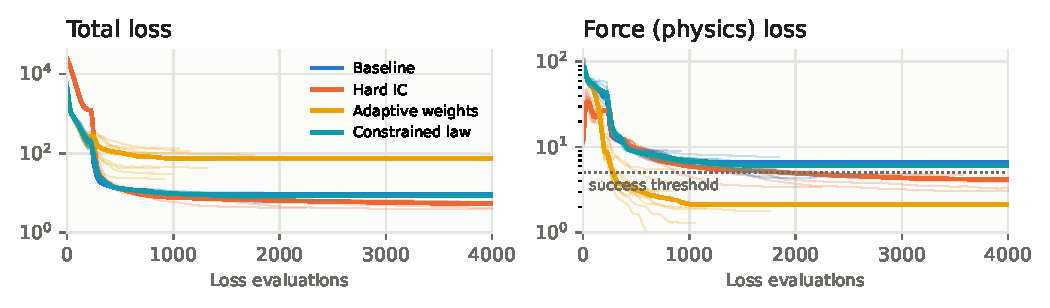
\includegraphics[width=\linewidth]{loss_curves.pdf}\vspace{-0.6em}
\caption{Training loss against loss evaluations (an L-BFGS step uses up to 20) for the four methods; faint lines are the 10 seeds, bold lines the median. The hard initial condition reaches the lowest loss; adaptive weights drive the force loss down while the total (trajectory-dominated) loss stays high.}
\label{fig:loss}
\end{figure}

\begin{figure}[t]
\centering
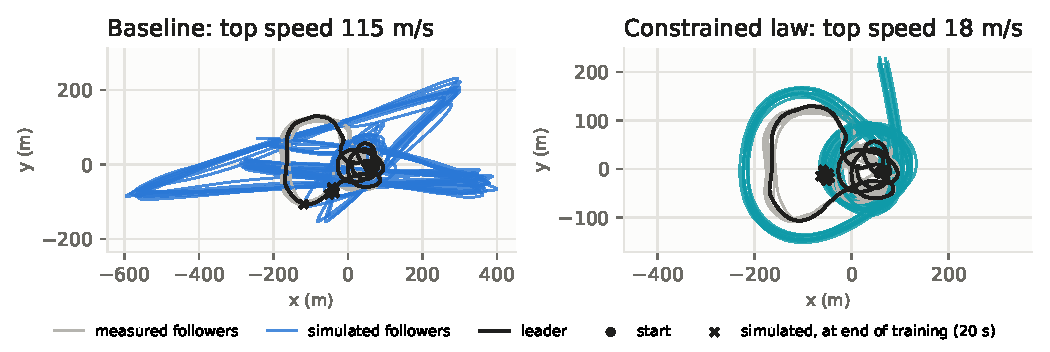
\includegraphics[width=\linewidth]{trajectories.pdf}\vspace{-0.6em}
\caption{Simulated flight paths (colour) against the measured followers (grey) over 18980--19120\,s, in the ground frame. Left: the baseline law that the original code returns (seed 3); followers are repeatedly slung several hundred metres out and back, at up to 115\,m/s. Right: the constrained law (same seed); the followers stay near the leader at realistic speeds (at most 18\,m/s; measured mean 12.4\,m/s), though on wider loops than the real birds.}
\label{fig:traj}
\end{figure}

\begin{figure}[t]
\centering
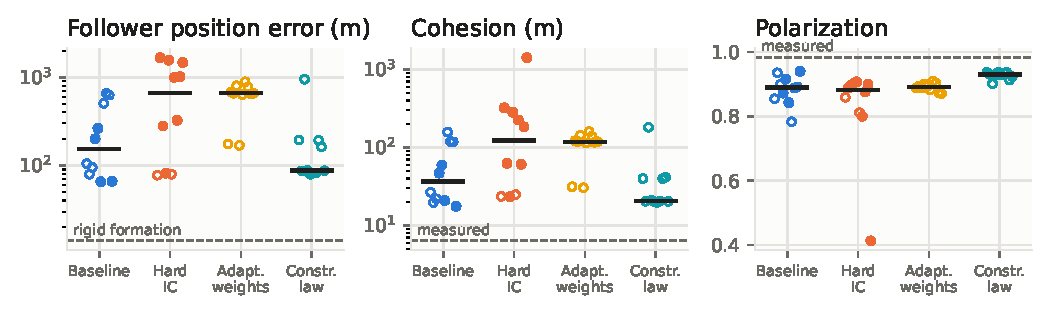
\includegraphics[width=\linewidth]{metrics.pdf}\vspace{-0.6em}
\caption{Simulation metrics over the unseen 20--140\,s for all 10 runs of each method (filled: passed the training success test; open: failed it; bar: median). Dashed lines: the rigid formation (left) and the measured flock (centre, right). Errors above about 400\,m mean the followers broke away from the leader.}
\label{fig:metrics}
\end{figure}

\section{Constraining the force law}\label{sec:constraints}
\textbf{Two failure modes.}
Simulating all baseline laws revealed two ways a learned law fails as a forward model.
(i)~\emph{Blow-up.} In the training window no two birds are more than 59\,m apart, so the fitted powers $\lambda_k d^{p_k}$ are pure extrapolation beyond it. A tiny coefficient on a high power costs nothing in training but dominates far out (baseline seed 4 has $-0.002\,d^{1.89}$, negligible at 10\,m but $-3$\,m/s$^2$ per neighbour at 60\,m). A bird that drifts 50--60\,m from the group is pulled back by nine such terms at once (25--30\,m/s$^2$), overshoots, and is pulled back harder from the far side; the only speed brake, $(|\bv v|-v_0)/\tau$, gives about 6\,m/s$^2$ even at 50\,m/s, so the cycle escalates (Fig.~\ref{fig:traj}, left). Of all laws simulated in this project, 9 of the 22 with $f(100\,\text{m})<-4$\,m/s$^2$ blew up, but only 1 of the 35 flatter ones.
(ii)~\emph{Break-away.} Followers fly 30--60\,m from the leader. Stable laws that pull weakly at that range let the followers keep together as a group but drift off in their own direction.

\textbf{Constraints.} Four changes target these mechanisms; the same constrained law is used in training and in the simulation (checked to agree to $10^{-6}$).
\begin{enumerate}\setlength{\itemsep}{1pt}
\item \emph{Bounded tail:} the distance laws are evaluated at a capped distance, $f\big(\min(d,d_c)\big)$ and $g\big(\min(d,d_c)\big)$ with $d_c=59$\,m, the largest training distance; the direction still uses the true distance.
\item \emph{Acceleration saturation:} each bird's summed interaction force is smoothly limited while its direction is kept,
\begin{equation}
\bv F_i\;\leftarrow\;a_{\max}\tanh\!\big(|\bv F_i|/a_{\max}\big)\,\hat{\bv F}_i,\qquad a_{\max}=10\ \text{m/s}^2,
\end{equation}
just above the largest measured follower acceleration (9.6\,m/s$^2$), so nine neighbours pulling together cannot exceed what a pigeon can do.
\item \emph{Minimum pull:} a penalty is added to the training loss when the distance force is less attractive than $-f_{\min}$ where followers actually fly,
\begin{equation}
\mathcal L=\mathrm{MSE}_x+\mathrm{MSE}_y+\mathcal L_F+\mu\,\frac{1}{|D|}\sum_{d\in D}\max\big(0,\,f(d)+f_{\min}\big)^2,\quad D=\{30,35,\dots,60\}\ \text{m},
\end{equation}
with fixed (not trained) $\mu=10$ and $f_{\min}=1.5$\,m/s$^2$, about half the leader's turning acceleration; averaging over the band penalises a dip anywhere in 30--60\,m. Capping the tail also removes the steep growth that, in the baseline, tethered stragglers to the leader; the penalty restores it at distances covered by data.
\item \emph{Own cruising speed:} each bird relaxes to its own mean measured speed $v_{0,i}$ (11.1--14.1\,m/s) instead of the flock mean. With a common $v_0$ the self-propulsion term pushes slow birds forward and fast birds back, a systematic error that the fitted interaction terms otherwise have to absorb.
\end{enumerate}

\begin{table}[t]
\centering\small
\caption{All 10 runs per method; simulation metrics over the unseen 20--140\,s (medians unless stated). $p$: Mann--Whitney test of the position errors against the baseline.}
\label{tab:results}
\begin{tabular}{lcccc}
\toprule
 & Baseline & Hard IC & Adaptive weights & Constrained law\\
\midrule
Training successes & 4/10 & \textbf{8/10} & 0/10 & 0/10\\
Final training loss & 8.82 & \textbf{5.34} & 73.1 & 8.48\\
Follower position error, median / best (m) & 153 / \textbf{65} & 660 / 78 & 657 / 169 & \textbf{88} / 80\\
$p$ against baseline & -- & 0.10 & 0.006 & 0.62\\
Runs with error $<150$ / 150--400 / $>400$\,m & 5 / 2 / 3 & 3 / 2 / 5 & 0 / 2 / 8 & \textbf{6} / 3 / \textbf{1}\\
Blow-ups (top speed $>50$\,m/s) & 2 & 8 & \textbf{0} & \textbf{0}\\
Cohesion (m; measured 6.3) & 37 & 123 & 119 & \textbf{21}\\
Polarization (measured 0.98) & 0.89 & 0.88 & 0.89 & \textbf{0.93}\\
\bottomrule
\end{tabular}
\end{table}

\textbf{Results.} Table~\ref{tab:results} and Fig.~\ref{fig:metrics} compare all runs.
The constraints remove both failure modes: none of the ten constrained flocks blows up (all stay below 35\,m/s), and only one breaks away, against two blow-ups and three break-aways for the baseline.
As a result the median follower position error drops from 153\,m to 88\,m, the flock is about half as spread (cohesion 21\,m vs.\ 37\,m) and better aligned (polarization 0.93 vs.\ 0.89), the best values of the four methods.
The training loss is essentially unchanged (8.48 vs.\ 8.82). No constrained run passes the success test, whose force-residual threshold the pull penalty competes with; that test did not predict simulation quality anyway (the failed baseline seeds 0--2 simulate better than the successful seeds 3 and 4).
The gains are in reliability rather than in the best case: the difference in errors is not significant over 10 seeds ($p=0.62$), the best constrained run (80\,m) does not beat the best baseline run (65\,m), and every law remains worse than the rigid formation (14\,m).
The pull penalty also fell short of its target: the weakest pull in the trained laws is $-1.0$ to $-1.2$\,m/s$^2$ rather than $-1.5$, because a weight of 10 is small against the data loss.

\section{Hard initial condition and adaptive weights}
\textbf{Hard initial condition (HIC).} The network output is replaced by a trial solution that satisfies the measured initial state exactly, $\bv r(t)=\bv r_0+\bv v_0 t+(t/T)^2 R\,\mathrm{NN}(t)$, with $T=20$\,s and $R=52.7$\,m the output scale of the original network; position and velocity at $t=0$ then equal the data, the same state the simulation starts from.
HIC does what it promises for training: 8 of 10 runs succeed (4 for the baseline) and the median loss falls from 8.82 to 5.34 (Fig.~\ref{fig:loss}).
But 8 of its 10 laws blow up in simulation and the median error rises to 660\,m.
Removing the initial-condition error lets the network fit the 20\,s trajectories more tightly, and the force coefficients follow every wiggle of that fit, with powers up to $d^{3}$, i.e.\ exactly the steep long-range tails identified in Section~\ref{sec:constraints}. A lower PINN loss is not a better flock model.

\textbf{Self-adaptive weights (AW).} Each loss term gets a weight $w=100\,\sigma(\lambda)$ (initially $\approx1$), and training solves $\min_{\theta}\max_{\lambda}\; w_d(\mathrm{MSE}_x+\mathrm{MSE}_y)+w_F\mathcal L_F$: Adam descends in the network and physics parameters $\theta$ while gradient ascent (rate 0.01) raises the weights of the terms that remain large. As the raw terms differ a hundredfold (about 7000 vs.\ 90), each weight's ascent gradient is divided by its term's initial value; the weights are frozen during L-BFGS, which needs a fixed objective.
Because the physics residual of a noisy, real flock cannot be driven to zero, the min--max rule kept raising $w_F$, and the growth fed on itself through the sigmoid's slope: $w_F$ reached 10--71 while $w_d$ stayed near 1.5.
The force loss then fell to about 2 at the expense of the trajectory fit (position MSE about 35, against 1.3), so the coefficients describe a flock that does not match the data: no run passes the success test and 8 of 10 flocks break away (median error 657\,m). A ten times smaller ascent rate keeps the weights near 1, i.e.\ the baseline.

{\footnotesize
\setlength{\bibsep}{0pt}
\bibliographystyle{unsrtnat}
\bibliography{references}
}
\end{document}
